\documentclass[10pt, a4paper]{article}

\usepackage[a4paper, top=2cm, bottom=2cm, left=2.2cm, right=2.2cm]{geometry}
\usepackage{amsmath, amssymb}
\usepackage{booktabs}
\usepackage{array}
\usepackage{tabularx}
\usepackage{multirow}
\usepackage{graphicx}
\graphicspath{{docs/Modification/}{./}}
\usepackage{hyperref}
\usepackage{enumitem}
%\usepackage{microtype}
\usepackage{parskip}
\usepackage{titlesec}
\usepackage{caption}
\usepackage{float}

\setlength{\parskip}{4pt}
\setlength{\parindent}{0pt}

\hypersetup{colorlinks=true, linkcolor=black, citecolor=black, urlcolor=black}

\titleformat{\section}{\normalsize\bfseries}{}{0em}{}%
  [\vspace{-4pt}\rule{\linewidth}{0.8pt}]
\titleformat{\subsection}{\normalsize\bfseries}{\thesubsection}{0.8em}{}
\titleformat{\subsubsection}{\normalsize\itshape}{\thesubsubsection}{0.8em}{}
\titlespacing{\section}{0pt}{10pt}{4pt}
\titlespacing{\subsection}{0pt}{6pt}{2pt}
\titlespacing{\subsubsection}{0pt}{4pt}{2pt}

\captionsetup{font=small, skip=4pt}

\begin{document}

% ── Header ───────────────────────────────────────────────────────────────────
\begin{center}
  {\large\textbf{MIS: Difficulty Scoring as a Pre-Augmentation Diagnostic
    for Agricultural Object Detection}}\\[4pt]
\end{center}
\rule{\linewidth}{1pt}
\vspace{2pt}

% ── Core claim ───────────────────────────────────────────────────────────────
\textbf{Claim (reframed from original draft).}
We propose: MIS a score that can provides structural diagnostics
 that identify the structural conditions underlying
copy-paste augmentation failure before augmentation is conducted.
The claim is not that MIS improves detection performance.
It changed to MIS exposes \emph{why} copy-paste fails on a given dataset,
which is useful before wasting compute on augmentation experiments.

\textbf{Why the claim changed.}
The original goal was to show MIS-guided copy-paste improves AP.
This belief was based on the research of Kisantal et al.\ \cite{kisantal2019},
When reanalyzing the result, i believe their success
relied on 2 specific conditions: (a) the MS COCO dataset with 3–5 objects per image on
average, (b) a two-stage Faster R-CNN with anchor-based RPN.
That make my assumstion that the method will work on different agricultural datasets has 
low chance of success. Because of that,
rather than searching for a positive result on a new dataset,
I chose to understand \emph{why} the failure is consistent and
whether MIS identifies that reason.

% ══════════════════════════════════════════════════════════════════════════════
\section{Methodology}
% ══════════════════════════════════════════════════════════════════════════════

\subsection{MIS Scoring}

Predictions generated at $\tau_{\text{conf}}=0.001$; matched to
ground truth at $\tau_{\text{IoU}}=0.5$.
The \textbf{object difficulty score}:
\begin{equation}
  S_{\text{obj}}(g) = \begin{cases}
    \min_{p \in \mathcal{P}(g)}
      \bigl[\alpha(1 - c_p) + \beta(1 - u_p)\bigr],
      & \mathcal{P}(g) \neq \varnothing \\
    \alpha + \beta = 1.0, & \text{missed object}
  \end{cases}
\end{equation}
$\alpha=\beta=0.5$, $c_p=\text{conf}(p)$, $u_p=\text{IoU}(p,g)$.
Taking the minimum removes noise from the many low-confidence candidates
generated at $\tau_{\text{conf}}=0.001$.

The \textbf{image difficulty score}:
\begin{equation}
  S_{\text{img}}(I) = w_1 \cdot \frac{1}{|G(I)|}
    \sum_{g \in G(I)} S_{\text{obj}}(g)
    + w_2 \cdot \text{FPrate}(I)
\end{equation}
$w_1=1$ (fixed). $w_2$ auto-calibrated by grid search to minimize
$|r(S_{\text{img}},\text{miss\_rate}) - r(S_{\text{img}},\text{FP\_rate})|$.

\subsection{MinneApple Dataset Split Problem and Fix}

\textbf{Problem I found late.}
MinneApple contains only 10 unique trees photographed at different times.
The test set was captured approximately one year after training.
A random 80/20 image-level split places images from the same tree in
both training and validation, causing the model to memorize tree-specific
features.
This inflated my baseline to AP\,$=0.439$ (contaminated; discarded).

\textbf{Fix.}
I try to implement the split that authors used on there original paper,
Tree-identity-clean split: 30 validation images from trees not in
training ($\approx$3 per held-out tree).
Training: 200 epochs max, early stopping patience 50.
Clean baseline: AP\,$=0.353 \pm 0.005$.


\subsection{MinneApple Size Thresholds}
As i analyse the Minne Apple dataset,
I see that the COCO thresholds (small $\leq32$\,px, medium $\leq96$\,px) do not suit
(traning set has no large objects and the test set has some of it which make the 
AP score following the size category not meaningful).
I define thresholds calibrated to the training distribution:

\begin{center}
\small
\begin{tabular}{lll}
\toprule
\textbf{Category} & \textbf{Criterion} & \textbf{Train \%} \\
\midrule
Very Small & area $\leq400$\,px$^2$ ($<20{\times}20$\,px) & 23.08\% \\
Small      & $400<$area$\leq1024$\,px$^2$ (20--32\,px)    & 50.53\% \\
Medium     & area$>1024$\,px$^2$ ($>32$\,px)              & 26.39\% \\
\bottomrule
\end{tabular}
\end{center}

\subsection{Augmentation Conditions}
Baed on the advices, I try a new method of copy and paste augmentation that 
is easier to analyze. 

First, all training images are ranked using the image-level 
difficulty score and divided into three equal 
groups: Score High, Score Medium, and Score Low. Depending on the 
experiment, images and objects are sampled from one of these groups.

To introduce some variation, each pasted object is randomly transformed 
with a scaling factor between 0.9 and 1.1, and a rotation of up to ±15 degrees.
The objects are pasted directly without any blending.
Training set extended by 30\% (189 synthetic images, same-image
constraint: objects pasted into their source image to preserve
photometric consistency.
Objects pasted: 2--8 per image, scale $[0.9,1.1]$, rotation $\pm15^\circ$,
no blending. \cite{kisantal2019}).
Each image can be selected for augmentation at most three times, 
and each object can also be reused at most three times across the entire dataset.

\begin{center}
\small
\begin{tabular}{lll}
\toprule
\textbf{Condition} & \textbf{Image pool} & \textbf{Object pool} \\
\midrule
Random        & Uniform random & Uniform random \\
Score High    & Top tertile    & Top tertile \\
Score Medium  & Middle tertile & Middle tertile \\
Score Low     & Bottom tertile & Bottom tertile \\
\bottomrule
\end{tabular}
\end{center}

Each condition: 3 seeds.

% ══════════════════════════════════════════════════════════════════════════════
\section{Score Validation}
% ══════════════════════════════════════════════════════════════════════════════

\subsection{Image-Level Correlation}

\begin{table}[H]
\centering\small
\caption{Pearson correlation of $S_{\text{img}}$ with per-image error rates.}
\begin{tabular}{lcc}
\toprule
\textbf{Dataset} & $r(\text{score, miss})$ & $r(\text{score, FP})$ \\
\midrule
MinneApple & 0.698 & 0.688 \\
GWHD 2021  & 0.816 & 0.818 \\
\bottomrule
\end{tabular}
\end{table}

Moderate-to-strong on both.
GWHD is higher because difficulty is structured at the domain level,
giving a cleaner signal.

\subsection{Object-Size Validity: MinneApple}

\begin{table}[H]
\centering\small
\caption{Mean $S_{\text{obj}}$ and baseline AP per size category.
  Consistent across all 3 seeds.
  Spearman $r_s=-0.82$: strong monotonic inverse relationship.}
\begin{tabular}{lcccc}
\toprule
\textbf{Category} & \textbf{AP} & \textbf{Mean $S$}
  & \textbf{Std} & \textbf{In top 30\% score tertile} \\
\midrule
Very Small & 0.071 & 0.1524 & 0.1433
  & \textbf{64.39\%} (5138 objects) \\
Small      & 0.270 & 0.0755 & 0.0475
  & 33.88\% (2704 objects) \\
Medium     & 0.493 & 0.0526 & 0.0184
  & \textbf{1.73\%} (138 objects) \\
\bottomrule
\end{tabular}
\end{table}

\textbf{My observation.}
98.27\% of high-difficulty objects are in size categories where
the model already performs poorly (AP $\leq 0.27$).
Only 1.73\% are in the medium category where the model has room
to improve.
This means score-guided augmentation, regardless of which difficulty
tier it targets, almost never selects objects in the learnable zone.
This is the key diagnostic finding on MinneApple.

\subsection{Domain-Level Validity: GWHD 2021 (18 domains)}

\textbf{Note on dataset version.}
I initially used a 7-domain subset of GWHD.
I re-ran on GWHD 2021 with 18 domains.
The correlation is stronger on the full dataset: Pearson $r=-0.905$,
Spearman $r_s=-0.899$.

\begin{table}[H]
\centering\small
\caption{GWHD 2021 domain analysis: MIS median difficulty vs.\ AP
  (18 domains, sorted by AP descending).
  MIS ranks all 18 domains correctly without domain labels.}
\begin{tabular}{lcr||lcr}
\toprule
\textbf{Domain} & \textbf{Med $S$} & \textbf{AP}
  & \textbf{Domain} & \textbf{Med $S$} & \textbf{AP} \\
\midrule
Arvalis\_10     & 0.200 & 0.744 & Arvalis\_8      & 0.342 & 0.546 \\
Rres\_1         & 0.227 & 0.658 & Arvalis\_5      & 0.342 & 0.542 \\
ETHZ\_1         & 0.268 & 0.643 & Arvalis\_9      & 0.372 & 0.520 \\
NMBU\_2         & 0.299 & 0.639 & Arvalis\_12     & 0.395 & 0.472 \\
Inrae\_1        & 0.264 & 0.633 & Arvalis\_3      & 0.350 & 0.470 \\
Arvalis\_11     & 0.358 & 0.606 & Arvalis\_7      & 0.407 & 0.463 \\
NMBU\_1         & 0.335 & 0.601 & Arvalis\_2      & 0.386 & 0.454 \\
Arvalis\_6      & 0.289 & 0.600 & Arvalis\_1      & 0.400 & 0.452 \\
ULiège-GxABT\_1 & 0.380 & 0.597 & Arvalis\_4      & 0.475 & 0.387 \\
\bottomrule
\end{tabular}
\end{table}

% ══════════════════════════════════════════════════════════════════════════════
\section{Augmentation Study}
% ══════════════════════════════════════════════════════════════════════════════

\subsection{MinneApple: Structural Bottleneck Pattern}

\begin{table}[H]
\centering\small
\caption{MinneApple: object scale distribution and 3-seed mean AP.
  All $\Delta$AP are within one standard deviation of baseline (ns).}
\begin{tabular}{lrrrrrr}
\toprule
\textbf{Condition} & \textbf{V.Small} & \textbf{Small}
  & \textbf{Medium} & \textbf{Gap} & \textbf{AP$\pm\sigma$}
  & $\Delta$\textbf{AP} \\
\midrule
Test target
  & 17.17\% & 38.14\% & 44.70\% & 0\,pp & --- & --- \\
\midrule
Baseline
  & 23.08\% & 50.53\% & 26.39\% & $-$18.31\,pp
  & 0.353$\pm$0.005 & --- \\
Random CP
  & 23.52\% & 49.98\% & 26.50\% & $-$18.20\,pp
  & 0.346$\pm$0.005 & $-$0.007 \\
Score High
  & 26.48\% & 49.59\% & 23.92\% & $-$20.78\,pp
  & 0.350$\pm$0.007 & $-$0.003 \\
Score Medium
  & 22.56\% & 50.80\% & 26.64\% & $-$18.06\,pp
  & 0.348$\pm$0.006 & $-$0.005 \\
Score Low
  & 19.99\% & 48.56\% & 31.45\% & $-$13.25\,pp
  & 0.348$\pm$0.003 & $-$0.005 \\
\bottomrule
\end{tabular}
\end{table}

\textbf{My observation on the Score Low result.}
Score Low achieves the largest distribution shift of any condition
(medium gap narrows from 18.31 to 13.25\,pp) yet produces no improvement.
This is the most informative result because it eliminates selection
strategy as the explanation.
Even when I select the easiest, most medium-sized objects,
the augmentation density increase is only 3.4\%
(42.57 $\to$ 44.03 objects per image).
On a dataset already averaging 42 objects per image,
a 3.4\% density increase is insufficient to shift model behavior.
The failure is a \textbf{structural bottleneck}, not a selection problem:
the dataset is too dense for copy-paste to add meaningful new signal.

This is in direct contrast to Kisantal et al.\ \cite{kisantal2019},
who achieved 30--60\% density increases starting from 3--5 objects
per image.
The mechanism that produced their gains cannot operate at MinneApple's
baseline density.

\textbf{Feature space confirmation.}
From image \ref{minneapple_feature_space}.

YOLOv8s P5 layer PCA centroids:
original train PC1$=+4.83$, augmented PC1$=+3.72$,
test PC1$=-11.24$.
Augmented images remain co-located with original training data
($\Delta\text{PC1}\approx 1.1$), both separated from test by
$\Delta\text{PC1}\approx 16$.
Copy-paste does not move the feature distribution toward the test set.

% Add image-level PCA plot showing original train, augmented train, and test distributions.
\begin{figure}[htbp]
\centering
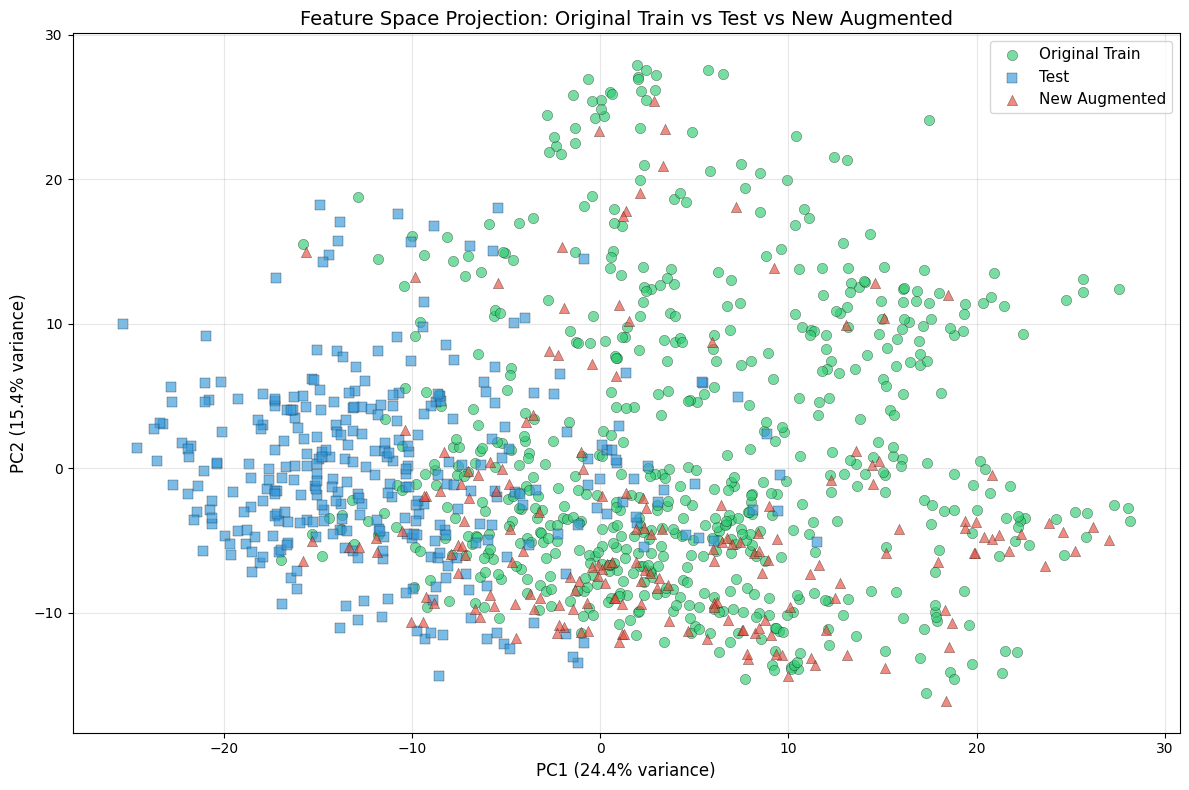
\includegraphics[width=0.98\linewidth]{minneapple_feature_space.png}
\caption{Feature space distribution of original training, augmented training, and test images in MinneApple.}
\label{minneapple_feature_space}
\end{figure}



\subsection{GWHD 2021: Stochastic Instability Pattern}

The GWHD results are qualitatively different from MinneApple
and reveal a second, distinct failure mode.

\begin{table}[H]
\centering\small
\caption{GWHD 2021 Score High augmentation results per seed
  (mean AP, Score High condition only).}
\begin{tabular}{lcc}
\toprule
\textbf{Seed} & \textbf{Baseline AP} & \textbf{Augmented AP} \\
\midrule
Seed 456 & 0.2126 &  0.2549  \textbf{+4.2 AP vs.\ baseline (helped)} \\
Seed 123 & 0.2307 & 0.1755   \textbf{$-$5.5 AP vs.\ baseline (hurt badly)} \\
Seed 789 & 0.2296 & 0.2239 ($-$0.6 AP, no effect) \\
\midrule
Mean $\pm$ std & 0.2296 & 0.2239 $\pm$ 3.98\% \\
\bottomrule
\end{tabular}
\end{table}

\textbf{My observation on GWHD seed variance.}
The ±3.98\% standard deviation across seeds is large relative to the
mean effect ($-$0.006 AP).
This is not random noise --- it is structurally caused.
MIS identifies that high-difficulty images in GWHD concentrate in
minority domains (Arvalis group, lowest AP).
When augmentation targets those images, it introduces training signals
dominated by a small number of underrepresented domains.
Whether that helps or hurts depends on which random seed determines
the sampling order, resulting in high-variance outcomes.

\textbf{Why this is different from MinneApple.}
On MinneApple, all five conditions converge to near-zero $\Delta$AP
with low seed variance ($\sigma \leq 0.007$).
The bottleneck is structural: density and resolution limits act
consistently regardless of seed.
On GWHD, the bottleneck is distributional: minority-domain concentration
creates inconsistent training signals that vary with sampling order.

\textbf{Important implication.}
For a practitioner: GWHD-type failure is actually \emph{worse} than
MinneApple-type failure.
A dataset with structural bottlenecks will consistently not improve;
you can measure this and move on.
A dataset with stochastic instability might improve with one seed and
fail badly with another --- the augmentation is unreliable rather than
simply ineffective.

% ══════════════════════════════════════════════════════════════════════════════
\section{Diagnostic Framework}
% ══════════════════════════════════════════════════════════════════════════════

\textbf{What this framework is and is not.}
The framework is a structured way to use MIS scores to reason about
whether copy-paste augmentation is likely to help, before running
any augmentation experiments.
It is \textbf{not a formal prediction system} with guaranteed accuracy.
The criteria were observed from two datasets (MinneApple and GWHD 2021)
and are retrospectively validated on the same data.
A prospective test on an unseen dataset would be needed to establish
it as a predictive tool.
I present it as an \emph{analytical checklist} for practitioners.

\subsection{The Three Structural States}

Rather than hard numerical thresholds (which would be arbitrary given
only two datasets), I frame each criterion as a qualitative structural
state that MIS can identify.

\medskip
\noindent\textbf{State 1 --- Information Bottleneck.}\\
\textit{Definition:} High-difficulty instances, as identified by MIS,
reside in a category where baseline AP is near zero.
This indicates a hardware/resolution limit rather than a representation
shortage: the model has no useful gradient to receive from these
instances regardless of how many times they appear in training.

\textit{How to check with MIS:}
\begin{enumerate}[nosep, leftmargin=*]
\item Compute $S_{\text{obj}}$ for all training objects.
\item Find the top-difficulty tertile.
\item Check what size/domain category dominates that tertile.
\item Look up the baseline AP for that category.
\item If AP is near zero --- the model fails on these objects
  almost completely --- this state is present.
\end{enumerate}

\textit{Action:} Copy-paste augmentation concentrated on high-difficulty
objects (Score High) will predominantly paste information-bottleneck
instances. \textbf{Score High augmentation is unlikely to help.}

\textit{MinneApple result:} 64.39\% of hard objects are very small
(AP$=0.071$). Information bottleneck state confirmed.

\medskip
\noindent\textbf{State 2 --- Stochastic Instability Risk.}\\
\textit{Definition:} High-difficulty images, as identified by MIS,
are concentrated in minority domains.
This means score-guided augmentation will disproportionately sample
from those domains, creating high-variance training signals whose
effect depends on sampling order.

\textit{How to check with MIS:}
\begin{enumerate}[nosep, leftmargin=*]
\item Find the top-difficulty tertile by $S_{\text{img}}$.
\item Check which domains those images come from.
\item If they are dominated by a small number of minority domains
  (domains with low domain-level AP), this state is present.
\end{enumerate}

\textit{Action:} Score-guided augmentation is not just unlikely to help ---
it introduces \textbf{high risk of stochastic instability}: results may
improve for some training seeds and degrade for others.
This makes augmentation \emph{unreliable} rather than simply ineffective.

\textit{GWHD 2021 result:} Hard images concentrate in Arvalis minority
domains. Stochastic instability confirmed: seed 456 $+4.2$\,AP,
seed 123 $-5.5$\,AP ($\sigma=3.98\%$).

\medskip
\noindent\textbf{State 3 --- Grid Saturation.}\\
\textit{Definition:} The dataset's baseline object density is high enough
that copy-paste augmentation at a standard ratio (e.g., 30\%) produces
a negligible proportional increase in object density.
When the baseline is already dense, pasting 5 more objects into an
image that already contains 42 does not meaningfully shift the
training distribution.

\textit{How to check (no MIS required):}
\begin{enumerate}[nosep, leftmargin=*]
\item Compute mean objects per image in the training set.
\item Estimate density increase:
  $\frac{\text{pasted objects per image} \times \text{augmentation ratio}}%
  {\text{mean objects per image}}$.
\item If the increase is small relative to baseline density,
  the dataset is in grid saturation for copy-paste at this ratio.
\end{enumerate}

\textit{Action:} Either significantly increase the augmentation ratio,
use cross-image paste (which this work did not test), or accept that
copy-paste cannot shift the distribution on this dataset at this ratio.

\textit{MinneApple result:}
$(5 \times 0.35) / 42.57 \approx 4.1\%$ density increase.
Score Low confirmed this: even the condition that moved the distribution
most (31.45\% medium vs.\ 26.39\% baseline) produced no AP improvement.

\subsection{Summary Diagnostic Table}

\begin{table}[H]
\centering\small
\caption{Applying the three structural states to MinneApple and GWHD 2021.
  All three states are present on both datasets.
  Predictions are consistent with experimental outcomes.}
\begin{tabular}{p{3.8cm}p{4cm}p{4cm}p{4cm}}
\toprule
\textbf{State} & \textbf{MinneApple} & \textbf{GWHD 2021}
  & \textbf{Observed} \\
\midrule
\textbf{Information Bottleneck:}
  hard objects near AP$=0$
  & 64.39\% of hard objects very small (AP$=0.07$).\newline
    State: \textbf{present}
  & AP varies by domain; not primary state.
  & \multirow{1}{=}{Structural bottleneck: consistent near-zero $\Delta$AP ($\sigma\leq0.007$)} \\[6pt]
\textbf{Stochastic Instability:}
  hard images in minority domains
  & Single domain dataset; not applicable.
  & Hard images in Arvalis minority group (lowest AP).\newline
    State: \textbf{present}
  & High variance: $\pm3.98\%$ across seeds \\[6pt]
\textbf{Grid Saturation:}
  negligible density increase
  & 4.1\% increase on 42.57 obj/img.\newline
    State: \textbf{present}
  & Similar pattern.
  & Distribution shift insufficient \\[6pt]
\midrule
\textbf{Overall prediction}
  & \textbf{Augmentation unlikely to help reliably}
  & \textbf{Augmentation unreliable (high variance)}
  & \textbf{Both confirmed} \\
\bottomrule
\end{tabular}
\end{table}

\subsection{When Copy-Paste Is Likely to Help}

The framework implies three conditions that together indicate
copy-paste augmentation is worth attempting:
(a) hard objects reside in a category where the model has partial
but not saturated performance --- neither near-zero nor already strong;
(b) high-difficulty images are spread across domains rather than
concentrated in a minority;
(c) augmentation meaningfully increases object density relative to
the baseline.

These conditions are consistent with Kisantal et al.'s success on COCO
and are absent on both MinneApple and GWHD 2021.

% % ══════════════════════════════════════════════════════════════════════════════
% \section{Response to Supervisor Suggestions}
% % ══════════════════════════════════════════════════════════════════════════════

% \textbf{``Sampling near the class boundary?''}\\
% I implemented difficulty-tier selection (tertile partitioning by
% $S_{\text{obj}}$), where Score Medium approximates sampling near the
% boundary between hard and easy objects.
% The result on MinneApple (Table 2): AP$=0.348\pm0.006$,
% $\Delta$AP$=-0.005$ (ns), similar to all other conditions.
% I note that my implementation is not identical to class-boundary
% sampling in the ML sense (which requires proximity to the
% decision boundary in confidence space, not in difficulty-score space).
% However, the result suggests that targeting the middle difficulty
% tier does not help on a dataset in the grid saturation state.

% \textbf{``Duplicating small samples?''}\\
% Yes, by design. The same-image constraint means all pasted objects
% come from the background image's own pool.
% With max\_object\_reuse$=3$, some objects are pasted multiple times.
% On MinneApple where images already average 42 objects, the
% within-image reuse adds transformed copies of objects the model
% has already seen in that scene.
% This adds positional diversity but no appearance diversity.
% I believe this is a contributor to the 3.4\% density ceiling ---
% the reuse cap limits how much the augmented dataset can diverge
% from the original.
% A cross-image paste experiment (same\_image\_only$=$False) would
% test whether removing this constraint changes the result.
% I did not run this due to time constraints.

% ══════════════════════════════════════════════════════════════════════════════
\section{Known Limitations and What I Would Do With More Time}
% ══════════════════════════════════════════════════════════════════════════════

\begin{enumerate}[nosep, leftmargin=*]
\item \textbf{Prospective validation.}
  The diagnostic framework was derived from the same datasets used to
  validate it.
  Testing it on a dataset where copy-paste is expected to help (e.g.,
  a sparse, single-domain dataset) and observing that the framework
  correctly identifies the absence of all three bottleneck states would
  substantially strengthen the claim.


\item \textbf{Threshold formalization.}
  The three structural states are described qualitatively.
  With more datasets spanning the full spectrum from failing to
  succeeding, the thresholds for each state could be derived
  statistically rather than by observation.
  With two failing datasets, no such derivation is valid.

\item \textbf{Using score with more advanced generative augmentation methods.}
  This work only tests copy-paste, but the diagnostic framework could
  be applied to other methods (e.g., generative models) that also have a
  selection component.
  It would be interesting to see if the same bottleneck states apply
  or if new ones emerge with different augmentation techniques.

\end{enumerate}

% ── References ───────────────────────────────────────────────────────────────
\begin{thebibliography}{9}

\bibitem{kisantal2019}
M.~Kisantal, Z.~Wojna, J.~Murawski, J.~Naruniec, and K.~Cho,
``Augmentation for small object detection,''
\textit{arXiv:1902.07296}, 2019.

\bibitem{ghiasi2021}
G.~Ghiasi et al.,
``Simple copy-paste is a strong data augmentation method for instance
segmentation,'' in \textit{Proc.\ IEEE/CVF CVPR}, 2021.

\bibitem{minneapple}
N.~Hani, P.~Roy, and B.~Bhanu,
``MinneApple: A benchmark for apple detection,''
\textit{IEEE RA-L}, vol.~5, no.~2, pp.~852--858, 2020.

\bibitem{gwhd}
E.~David et al.,
``Global Wheat Head Detection (GWHD) dataset,''
\textit{Plant Phenomics}, 2021.

\bibitem{ohem}
A.~Shrivastava, A.~Gupta, and R.~Girshick,
``Training region-based object detectors with online hard example mining,''
in \textit{Proc.\ IEEE CVPR}, 2016.

\bibitem{focal}
T.-Y.~Lin et al.,
``Focal loss for dense object detection,''
in \textit{Proc.\ IEEE ICCV}, 2017.

\bibitem{yolov8}
G.~Jocher et al., ``YOLO by Ultralytics,'' v8.0.0, 2023.

\end{thebibliography}

\end{document}
